\documentclass[12pt, letterpaper]{article}
\usepackage{graphicx} % Required for inserting images
\usepackage{hyperref}
\usepackage{listings}
\usepackage{amssymb}
\usepackage{amsmath}
\usepackage[english]{babel}
\usepackage{nicefrac, xfrac}
\usepackage{mathtools}
\usepackage[table,xcdraw]{xcolor}
\definecolor{light-gray}{gray}{0.95}
\definecolor{sap}{RGB}{130, 36, 51}
\definecolor{lg}{RGB}{102, 161, 95}
\usepackage[paper=a4paper,left=20mm,right=20mm,bottom=25mm,top=25mm]{geometry}
\newcommand{\code}[1]{\colorbox{light-gray}{\texttt{#1}}}
\newcommand{\shelll}[1]{\colorbox{black}{\textcolor{white}{\texttt{#1}}}}
\newcommand{\shell}[1]{\colorbox{black}{\textcolor{white}{\texttt{casufrost@debian:$\sim$\$ #1}}}}
\newcommand{\codee}[1]{\colorbox{white}{\texttt{#1}}}
\newcommand{\acc}{\\\hphantom{}\\}
\newcommand{\dete}{{\rightarrow}}
\newcommand{\fdot}{{\(\bullet\) }}
\newcommand{\boxedMath}[1]{\begin{tabular}{|c|}\hline \texttt{#1} \\ \hline\end{tabular} :}
\title{Reti di Elaboratori}
\author{Marco Casu}
\date{\vspace{-5ex}}
\begin{document}



\maketitle
\begin{figure}[h]
    \centering{
    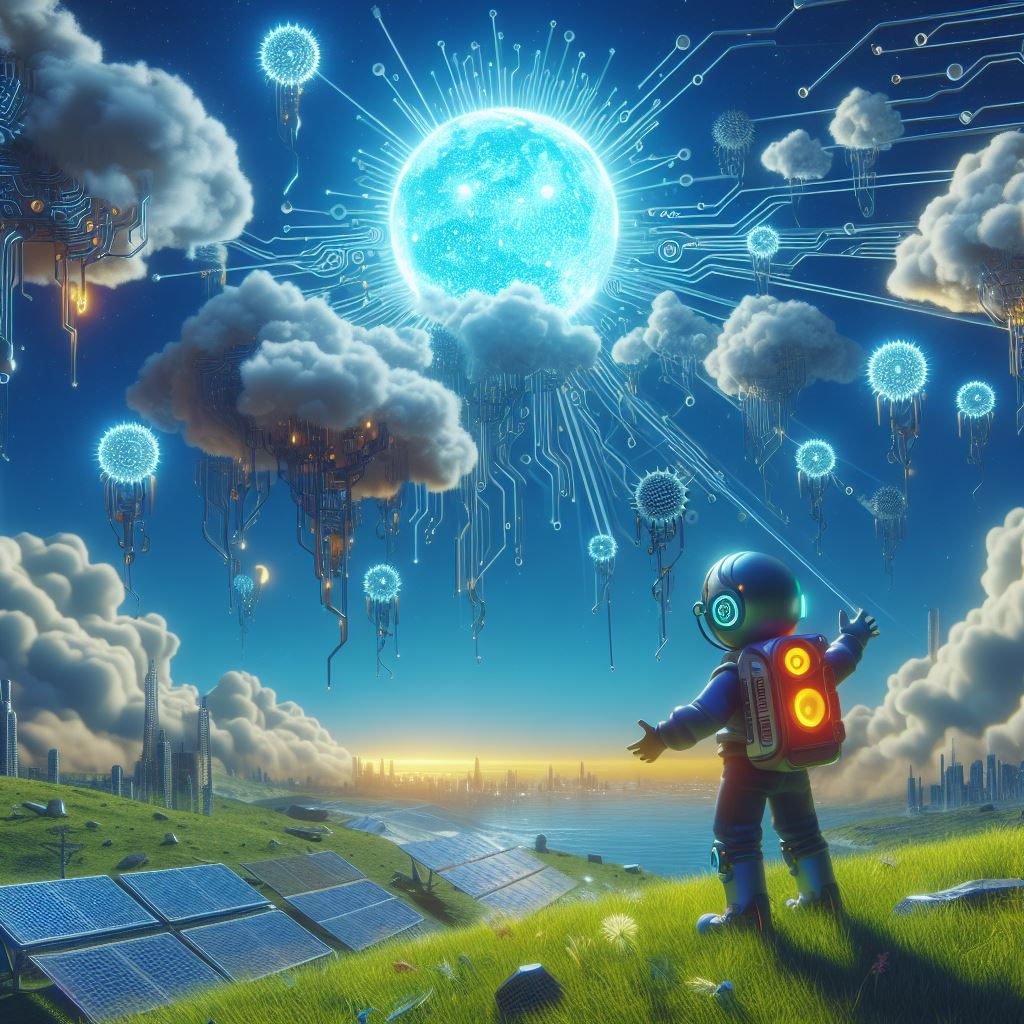
\includegraphics[width=1\textwidth ]{images/cop.jpg}
    }
\end{figure}
\newpage 
\tableofcontents
\newpage
\section{Introduzione e Definizioni}
Cos'è una richiesta di rete? E soprattutto quali sono i passaggi ed il procedimento scaturito a seguito di una richiesta? Questo corso 
si concentrerà sull'aspetto del \textit{networking}, ossia, su come avviene la comunicazione tramite più elaboratori.\acc 
Una \textit{connessione} è una comunicazione aperta in cui sono coinvolte entrambe le parti in attesa di ricevere ed inviare 
messaggi, tramite l'apertura di un \textit{socket} (si approfondirà in seguito). Il problema di una comunicazione di questo tipo, 
è il bisogno di avere la certezza che i messaggi inviati da una parte siano ricevuti correttamente dall'altra, senza il rischio di 
comunicare "a vuoto", per questo sono definiti degli appositi protocolli.\acc 
\textbf{Host} : Un dispositivo connesso alla rete in modo periferico, non funge da esclusivo tramite per la comunicazione, 
ed è un sistema "periferico", esegue delle \textit{app} che forniscono servizi sulla rete.\acc 
\textbf{Switch} : Gli switch sono i dispositivi capaci di "instradare" i \textit{pacchetti}.\acc
\textbf{Rete} : Una collezione di dispositivi host/switch e collegamenti gestiti da un unico ente/organizzazione.\begin{center}
    \includegraphics[width=1\textwidth ]{images/reteDef.eps}
\end{center}
Quella che noi chiamiamo \textbf{internet}, è una "\textit{rete di reti}", ossia l'insieme interconnesso di tutte le reti 
pubbliche, che si stabilisce e necessita di protocolli su tutti i livelli : \begin{itemize}
    \item Livello di applicazione
    \item Livello di trasporto 
    \item Livello network 
    \item Livello di collegamento
\end{itemize}
Lo scopo di internet è quello di essere un infrastruttura che fornisce i servizi alle applicazioni distribuite, è 
un interfaccia di programmazione e fornisce un servizio di \textit{trasporto dei dati}.\acc 
Un \textbf{protocollo di rete}, stabilisce delle regole riguardanti lo scambio di messaggi, con le relative "azioni" specifiche 
da intraprendere per la ricezione di messaggi ed eventi, definiscono il \textit{formato} e \textit{l'ordine} dei messaggi 
da inviare fra le entità di rete, e le azioni intraprese sulla ricezione e trasmissione dei messaggi.
\subsection{Struttura di Internet e Link}  
Una rete è quindi un insieme di nodi collegati tramite dei \textit{link}, composta da dispositivi di interconnessione, che 
si scambiano informazioni, usualmente utilizziamo il termine \textit{host} per i dispositivi che usufruiscono di un servizio, 
e \textit{server} per i dispositivi che lo erogano.\acc 
I dispositivi di interconnessione, ricevono un segnale, lo modificano e lo ritrasmettono, sono i \textit{router} (collegano una 
rete ad altre reti) e gli  \textit{switch} (collegano più dispositivi ad una rete locale). I collegamenti, o link, possono 
essere cablati (rame o fibra ottica) oppure wireless, senza cavi (onde elettromagnetiche).\acc 
Le reti locali come quelle casalinghe o aziendali, si collegano ad una rete regionale ISP (internet service provider) di router interconnessi detta 
\textit{core} o \textit{backbone}, che a sua volta si collega ad una simile struttura ma a livello nazionale o globale.\acc 
\subsubsection{Reti Cablate e Wireless}
Nell'accesso via cavo, c'è un terminale comune per più abitazioni detto \textbf{CMTS}, ossia \textit{Cable Modem Termination System},
che viene poi diramato nelle diverse abitazioni, i dati dalla rete ed i segnali per la televisione sono trasmessi sul medesimo 
cavo ma a frequenze differenti. Il CMTS è direttamente collegato ad un ISP. In questo modello diverse case condividono la rete di 
accesso.\begin{center}
    \includegraphics[width=1.1\textwidth ]{images/cableHeadend.eps}
\end{center}
La \textbf{DSL} diversamente, utilizza la linea telefonica esistente, collegandosi alla DSLAM, i dati sulla linea 
DSL vanno su internet, la voce su DSL va sulla linea telefonica. \acc 
Una rete \textit{domestica}  c'è un \textit{modem} 
(si occupa di ricevere il segnale analogico e di  \textit{modularlo} in segnale digitale)
 connesso ad un CMTS, collegato via cavo ad 
un router, collegato direttamente tramite \textit{ethernet} agli host, oppure collegato ad un \textit{access point WI-FI} che 
permette la connessione senza fili, questi utlimi tre molto spesso sono combinati in un unico device.\acc 
La connessione senza fili, o wireless connette i sistemi terminali (host) al router, tramite il già citato 
access point, esistono reti locali senza fili (WLAN), che hanno una copertura di circa 30 metri, e reti di accesso 
cellulare \textit{wide area}, utilizzate dai dispositivi mobili e fornite da un operatore di rete cellulare, ed hanno una 
copertura più ampia, nell'ordine dei kilometri.\acc 
Le reti aziendali, come quelle delle università sono di una scala diverso rispetto quelle domestiche, prevedono molti più 
dispositivi, ed un mix di varie tecnologie di collegamento, cablate o wireless, tramite svariati switch e router.
\subsubsection{Comunicazione e Classificazione delle Reti}
Un host comunica tramite l'invio e la ricezioni di messaggi da un applicazione sottoforma di \textit{pacchetti} di dati, ossia 
messaggi suddivisi in blocchi più piccoli, di lunghezza $L$ bit. L'host trasmettono i pacchetti nella rete 
ad una \textit{velocità di trasmissione} di $R$ $\nicefrac{bit}{sec}$. Il \textit{ritardo} di trasmissione del pacchetto è 
il tempo necessario per trasmettere il pacchetto ($L$ bit) nel collegamento, ed equivale a $\dfrac{L}{R}$ secondi.\acc 
Il segnale si propaga fra trasmettitore e ricevitore, tramite \textit{supporti guidati}, ossia i mezzi solidi (cavi), oppure 
 \textit{non guidati}, propagandosi liberamente nell'aria (onde elettromagnetiche).\begin{itemize}
    \item Il \textbf{cavo coassiale} è provvisto di due conduttori di rame concentrici, è bidirezionale, supporta più canali
    date diverse frequenze, ed è resistente alle interferenze. 
    \item La \textbf{fibra ottica} ha soppiantato il cavo coassiale, è una fibra di vetro che trasporta impulsi luminosi, dove ciascun 
    impulso rappresenta un bit, la luce rimbalza nel cavo muovendosi ad alta velocità, è necessario però considerare dei 
    ripetitori (anche se molto distanziati), dato che la luce rimbalzando potrebbe tendere a disperdersi causando una perdita 
    di informazioni.
    \item La rete \textbf{wireless} non ha un supporto guidato, il segnale è propagato nell'aria, è quindi \textit{broadcast},  
    chiunque può ricevere il segnale. Tale metodo di comunicazione è \textit{half-duplex}, ossia, la comunicazione avviene da un 
    mittente ad un destinatario, e non è possibile comunicare fra due enti contemporaneamente, è soggetta ad effetti dovuti all'ambiente 
    di propagazione, come interferenze, riflessione e ostruzione da parte di oggetti fisici.
 \end{itemize}
 Esiste una scala di classificazione delle reti :\begin{center}
    \begin{tabular}{|
        >{\columncolor[HTML]{EFEFEF}}c |
        >{\columncolor[HTML]{FFFFFF}}c |c|
        >{\columncolor[HTML]{FFFFFF}}c |}
        \hline
        \cellcolor[HTML]{9AFF99}{\color[HTML]{000000} Scala} & \cellcolor[HTML]{9AFF99}Tipo & \cellcolor[HTML]{9AFF99}Nome completo & \cellcolor[HTML]{9AFF99}Esempio \\ \hline
        Distanza ravvicinata                                 & PAN                          & Personal Area Network                 & Bluetooth                       \\ \hline
        Edificio                                             & LAN                          & Local Area Network                    & WiFi, Ethernet                  \\ \hline
        Città                                                & MAN                          & Metropolitan Area Network             & Cablata, DSL                    \\ \hline
        Paese                                                & WAN                          & Wide Area Network                     & Grandi ISP                      \\ \hline
        Pianeta                                              & Internet                     & La rete di tutte le reti              & L'Internet                      \\ \hline
        \end{tabular}
 \end{center}
 La \textbf{LAN} è la rete locale, come una rete domestica, è una rete privata ed ogni terminale connesso ad essa è identificato 
 da un indirizzo distinto dagli altri, può essere a \textit{cavo condiviso} oppure a \textit{commutazione} con uno switch.\begin{center}
    \includegraphics[width=1\textwidth ]{images/cavocondiviso.eps}
\end{center}
In tale modello di cavo condiviso il pacchetto inviato ad un dispositivo viene ricevuto da tutti, solo il destinatario lo 
elaborerà, tutti i restanti host lo ignoreranno.\acc \begin{center}
    \includegraphics[width=0.7\textwidth ]{images/commutazione.eps}
\end{center}
Quest'ultimo a commutazione è il più utilizzato tutt'oggi, ogni dispositivo è direttamente collegato allo switch, ed esso è 
in grado di riconoscere gli host ed inviare i pacchetti esclusivamente al destinatario, riduce il traffico nella LAN.\acc 
Le reti \textbf{WAN} sono reti geografica, vengono interconnessi dispositivi di comunicazione, necessari a città, regioni o 
perfino nazioni. I dispositivi in questione sono switch, router e modem, tale rete è gestita da un grande operatore/ente di 
telecomunicazioni detto IPS (Internet Service Provider) che fornisce i servizi alle organizzazioni.\acc Una WAN può vedere i suoi 
dispositivi di comunicazione connessi punto-punto, oppure a commutazione, con più punti di terminazione (usata nelle dorsali di 
Internet), tutt'oggi è raro trovare LAN o WAN isolate, spesso sono connesse fra loro per formare una internetwork (internet), per 
mettere in comunicazione due LAN in città differenti tramite una WAN.\begin{center}
    \includegraphics[width=1\textwidth ]{images/internetwork.eps}
\end{center}
\subsubsection{Nucleo della Rete}
Si definisce nucleo della rete, quella parte composta esclusivamente da router  che effettuano \textit{commutazione} di pacchetto, ossia 
ricevono il pacchetto, e lo re-indirizzano tramite i collegamenti. Ogni router presenta più porte, si occupa di fare il 
cosiddetto \textbf{forwarding}, ossia l'azione locale di spostare i pacchetti in arrivo dal collegamento in ingresso, al collegamento 
in uscita, è un azione locale del router.\acc 
Il \textbf{routing} invece è un azione globale, si intende la determinazione dei percorsi origine-destinazione che i pacchetti 
dovranno prendere all'interno dell'Internet, tale decisione è presa tramite degli algoritmi di instradamento.\acc 
Con il termine \textit{Trasmissione}, si intende l'azione che intraprende un pacchetto per essere trasferito interamente 
sul collegamento. Tale termine non include l'intero tragitto fino a destinazione, ma esclusivamente la (appunto) trasmissione sull'eventuale 
cavo, il \textit{ritardo di trasmissione} è quindi il delay misurato in secondi per trasmettere un pacchetto, si è già specificato che tale 
valore è uguale a $\dfrac{L}{R}=\dfrac{\text{bit di un pacchetto}}{\text{bit per secondo}}$.\acc 
I router funzionano nella seguente maniera, detta \textbf{store and forward} : Un pacchetto deve arrivare per intero ad un router 
prima di essere ri-trasmesso su un nuovo collegamento.\begin{quote}
    \color{gray} \textit{Esempio} : Si devono trasferire, dal collegamento A al collegamento B, 3 pacchetti da 10 Kbit ad una 
    velocità di 100 Mbitt per secondo, si assume che il  tempo che impiega un bit per propagarsi nel collegamento è zero. 
    In totale, il ritardo di trasmissione sarà : $\dfrac{10*3*10^3}{100*10^6}=\dfrac{3}{100*10^2}=\dfrac{3}{10^4}=0,0003\text{ sec }=0,3\text{ msec }$
    \color{black}
\end{quote}
Un problema noto durante la tramissione dei pacchetti è l'\textbf{accodamento}, avviene quando la velocità di arrivo ad 
un router da parte di un link è maggiore della velocità di trasmissione in uscità (dal link al router), quindi si causa un 
accodamento in attesa della trasmissione.\begin{center}
    \includegraphics[width=0.7\textwidth ]{images/accodamento.ip.eps}
\end{center}
I pacchetti arrivano al router prima di essere trasmessi sul link, quindi si accoderanno in una memoria interna del router prima 
di essere ritrasmessi, se i pacchetti accodati diventano troppi e la memoria viene esaurita, ci sarà una \textit{perdita} di 
pacchetti. \acc 
Una possibile soluzione alla perdita è la \textbf{commutazione di circuito}, ossia, far si che i diversi host non condividano lo 
stesso collegamento per i pacchetti, bensì, si considerano dei canali riservati per la comunicazione tra sorgente e destinazione.\acc 
Non c'è condivisione, ci saranno quindi svariati collegamenti, in numero necessario per permettere a tutti i dispositivi di 
poter comunicare in modo libero, ovviamente non tutti comunicano nello stesso momento, quindi i un segmento di cirucito potrebbe 
rimanere inutilizzato.\acc 
Un'altra alternativa è quella di condividere lo stesso circuito, riservando ad ogni comunicatore una frequenza (\textit{FDM}), oppure un certo 
quanto temporale (\textit{TDM}).\begin{itemize}
    \item Nel FDM, le frequenze elettromagnetiche o ottiche sono divise in bande, ogni utente può comunicare in maniera continua, 
    ma la velocità massima di comunicazione è data dalla larghezza della banda, che è stretta in quanto condivisa.
    \item Nel TDM, ogni utente, a turno in un attesa circolare, può comunicare per un quanto di tempo determinato, in cui ha a 
    disposizione la velocità massima della banda.
\end{itemize}\begin{center}
    \includegraphics[width=1\textwidth ]{images/FdmTdm.eps}
\end{center}
Il problema è che la commutazione di circuito risulta comunque in efficiente, in quanto permette ad un numero 
limitato di utenti di usufruire della rete. Si preferisce quindi la condivisione delle risorse, in quanto l'accodamento e la 
significativa perdita di pacchetto, incombe quando un elevato numero di utenti sta usufruendo della rete.\acc 
Il fatto è che gli utenti non comunicano il 100\% del tempo, supponiamo che un utente stia comunicando con probabilità $p$, in un 
sistema con $n$ utenti. Vi è una significativa perdita di pacchetto quando $k$ utenti condividono le risorse, qual'è la probabilità che 
$k$ utenti comunichino contemporaneamente ?\acc  Sia $X$ la variabile aleatoria che indica il numero di utenti che comunica 
contemporaneamente, $X$ è una variabile aleatoria binomiale, e la sua distribuzione vale
 $\displaystyle\mathbb{P}(X\ge k)=\sum_{i=k}^n\binom{n}{i}p^i(1-p)^{n-i}$.\begin{quote}
 \color{gray} \textit{Esempio} : In un sistema con 35 utenti, ogni utente comunica con probabilità uguale a 0.1. 
 Vi è una significativa perdita di pacchetto quando 10 utenti comunicano contemporaneamente, qual'è la probabilità che 
 ciò accada? $$\sum_{i=10}^{35}\binom{35}{i}(0.1)^i(0.9)^{35-i}\simeq0.001$$
 \color{black}
\end{quote}
La condivisione del circuito risulta quindi la scelta migliore, anche se la possibile congestione in casi particolari 
è eccessiva, e risulta inevitabilmente una perdita di pacchetti.\subsubsection{Internet}
Fino ad ora, abbiamo utilizzato il termine Internet (con la iniziale maiuscola) ed internet (con la iniziale minuscola), è necessario 
dare una definizione più rigorosa di Internet.\acc 
Abbiamo visto come gli host si connettono ad Internet tramite l'accesso agli ISP, residenziali o aziendali. I grandi ISP sono fra 
loro interconnessi, da qui il nome internet (inter network), in tal modo, tutti gli host connessi ai differenti ISP possono 
scambiarsi pacchetti.\acc Ogni host connesso ad Internet, è quindi connesso ad un ISP, ed i grandi ISP sono tutti interconnessi fra loro, 
creando un unica grande rete globale, denominata appunto, Internet (con la iniziale maiuscola), ossia una rete delle reti.\acc 
Tale rete globale è complessa, e la sua evoluzione, nella struttura, è anche derivata da dinamice politiche ed economiche a livello 
nazionale, si osservi la seguente immagine.\begin{center}
    \includegraphics[width=1\textwidth ]{images/Internet.eps}
\end{center}
Le icone con scritto \textit{accesso rete} rappresentano i punti in cui un host può connettersi, ad esempio una LAN, tali punti si 
collegano agli ISP regionali, che a loro volte si collegano ad ISP nazionali, spesso condiviso anche da più nazioni, spesso 
interconnessi da degli \textit{Internet Exchange Point} (ISP), gestiti da più enti in comune accordo.\acc Quindi una 
internet è una rete costituita da più reti interconnesse, Internet invece, è la "internet" più grande e famose, composta da migliaia di reti 
interconnesse.
\end{document}
